%In dit hoofdstuk moet het volgende besproken worden:
%-Uitleggen van het probleem
%-Hoe ik tewerk ga gaan
%-Gaan we concluderen met de onderzoeksvraag
\chapter{Situering}\label{hfdst:situering}
Televic Rail heeft een Python test framework ontworpen waarmee zij in staat zijn om verschillende hardware componenten te controleren op fouten.
Dit framework wordt dan ook zeer intensief gebruikt tijdens het productieproces.
Het framework werd initieel ontworpen om enkel te werken op testtorens, maar werd later aangepast zodanig dat het onafhankelijk van de testtoren gebruikt kan worden.

\section{Het probleem}\label{sec:probleem}
Aangezien het Python framework gebruikt van verschillende niet-Python bibliotheken en verschillende drivers voor de hardware, is het installeren van dit framework op een nieuw systeem een ganse klus.
Updates uitvoeren geeft ook verschillende problemen.
Het doel van deze thesis is dan ook het vinden van een langdurige oplossing van dit probleem.
Na een kleine analyse van het probleem, werd het al snel duidelijk dat er op verschillende onderliggende problemen een oplossing moet gevonden worden.

Het framework bestaat uit verschillende componenten en drivers.
Al deze componenten en drivers hebben hun eigen installatie wijze en moeten in een bepaalde volgorde geïnstalleerd worden.
Hiernaast hebben sommige doelsystemen een specifiek configuratiebestand nodig om goed te kunnen functioneren.
Tijdens deze thesis zal er dan ook onderzocht worden hoe alle verschillende componenten kunnen worden gepackaged tot één groot geheel dan kan worden verzonden naar de verscheidene doelsystemen.

De installatie van het framework gebeurt best in een speciale deployment omgeving.
Mocht er een fout optreden tijdens de installatie, of tijdens een update, van het framework, dan moet een vorige, nog werkende, versie van het framework herstelt worden.
Hierdoor voorkomen we verschillende problemen, zoals het stilleggen van de productie.
Er moet dus onderzocht worden of het mogelijk is om een omgeving te creëren waarin een update/installatie kan plaatsen vinden en, mocht dit nodig zijn, de aanpassingen kunnen ongedaan worden gemaakt.

Naast het updaten/installeren zijn er nog problemen.
Het framework wordt gebruikt op verschillende sites en niet ieder site zal dezelfde versie van het framework gebruiken.
Bij een rollout van een nieuwe versie is het mogelijk dat de update slaagt in de ene site maar niet op de andere.
Het bijhouden van de verschillende, al dan niet geslaagde, deployments moeten centraal zichtbaar zijn.
Om die redenen zal er onderzocht moeten worden om een overkoepelende manager te voorzien.
Met deze manager kan er een overzicht gecreëerd worden waarmee zichtbaar wordt welke deployments geslaagd zijn, hoeveel updates gelukt zijn, de versie van het framework dat gebruikt wordt op één bepaalde site, \ldots .
Dit onderdeel moet zeer schaalbaar zijn zodanig dat naar de toekomst toe, het zeer eenvoudig is om nieuwe systemen toe te voegen.

\section{Werkwijze}
In Sectie~\ref{sec:probleem} heb ik besproken welke verschillende problemen opgelost moeten worden.
In wat volgt ga ik bespreken hoe ik dit ga aanpakken en op welke wijze ik te werk ga gaan.

Tijdens de bespreking van de problemen werd het al snel duidelijk dat het werk op te delen valt in drie grote componenten.
De oplossing die opgebouwd wordt tijdens deze thesis zal dan ook uit deze drie componenten bestaan en alle verschillende stappen worden uit gelegd aan de hand van deze drie onderdelen.
Het eerste onderdeel is de packager.
Deze component zal instaan voor het inpakken van de verschillende drivers en zal ook de software bevatten die het installatieproces in goede banen zal leiden.
Naast de packager hebben we dan de deployment server.
De server zal functioneren als manager in het grote geheel met als doel het weergeven van alle verschillende deployments en verschillende gegevens, zoals bijvoorbeeld de versie van het framework.
Het laatste onderdeel dat voorzien zou moeten worden is dan de deployment omgeving.
De omgeving draait op de verschillende systemen en zal dienen als een sandbox voor het installeren/updaten van het framework.

Verder gaat deze thesis nog onderverdeelt worden in twee grote delen.
In het eerste deel gaat er een prototype worden gemaakt met de bovengenoemde elementen.
Als het prototype gemaakt is, zal het systeem getest worden en zal er gecontroleerd worden of alle nodige componenten goed geïmplementeerd werden.
Na deze stap zal het ontwerp aangepast worden en zal de einde demo gemaakt worden.
De laatste fase van deze thesis bestaat dan uit het testen van deze demo waarna het dan mogelijk is om een conclusie te trekken uit het geleverde werk.

\begin{figure}[!h]
\centering
  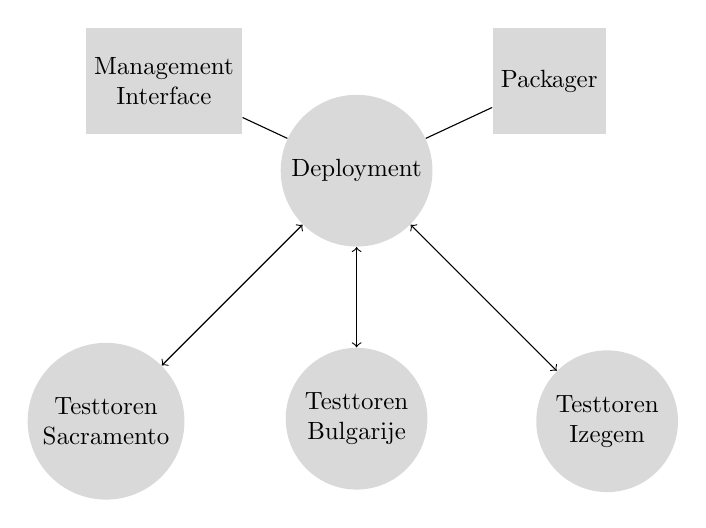
\begin{tikzpicture}[scale=.9, transform shape]
\tikzstyle{every node} = [circle, minimum size = 2cm, fill=gray!30]
\node (a) at (0, 0) {Deployment};
\node[shape = rectangle,minimum size = 1.5cm] (packager) at +(25: 3) {Packager};
\node[shape = rectangle,minimum size = 1.5cm, align=center] (logger) at +(155: 3) {Management\\ Interface};
\node[align=center] (b) at +(225: 5) {Testtoren\\ Sacramento};
\node[align=center] (c) at +(270: 3.5) {Testtoren\\ Bulgarije};
\node[align=center] (d) at +(315: 5) {Testtoren\\ Izegem};
\foreach \from/\to in {a/b, a/c, a/d}
\draw [<->] (\from) -- (\to);
\draw [-] (a) -- (packager);
\draw [-] (a) -- (logger);
\end{tikzpicture}
  \caption{My TikZ picture}
  \label{fig:overzichtDiagram}
\end{figure}

\begin{figure}[!h]
\centering
  % We need layers to draw the block diagram
\pgfdeclarelayer{background}
\pgfdeclarelayer{foreground}
\pgfsetlayers{background,main,foreground}

% Define a few styles and constants
\tikzstyle{sensor}=[draw, fill=blue!20, text width=5em, 
    text centered, minimum height=2.5em]
\tikzstyle{ann} = [above, text width=5em]
\tikzstyle{naveqs} = [sensor, text width=6em, fill=red!20, 
    minimum height=12em, rounded corners]
\tikzstyle{naveqq} = [sensor, text width=6em, fill=red!20, 
    minimum height=2.5em, rounded corners]
\def\blockdist{2.3}
\def\edgedist{2.5}

\begin{tikzpicture}
    \node (packagerServer) [naveqs] {Packager Interface};
    % Note the use of \path instead of \node at ... below. 
    \path (packagerServer.140)+(-\blockdist,0) node (gyros) [sensor] {Rapport};
    \path (packagerServer.-150)+(-\blockdist,0) node (collect) [sensor] {Data Collector};
    
    % Unfortunately we cant use the convenient \path (fromnode) -- (tonode) 
    % syntax here. This is because TikZ draws the path from the node centers
    % and clip the path at the node boundaries. We want horizontal lines, but
    % the sensor and naveq blocks aren't aligned horizontally. Instead we use
    % the line intersection syntax |- to calculate the correct coordinate
    % We could simply have written (gyros) .. (naveq.140). However, it's
    % best to avoid hard coding coordinates
    \path [draw, ->] (collect) -- node [left] {info} 
        (collect.north |- gyros.south);
    \path [draw, <-] (collect) -- node [below] {info} 
        (packagerServer.west |- collect);    
    \node (IMU) [above of=gyros] {Status};
    \path (packagerServer.south west)+(-0.6,-0.4) node (INS) {Deployment Server};
    
    % Now it's time to draw the colored IMU and INS rectangles.
    % To draw them behind the blocks we use pgf layers. This way we  
    % can use the above block coordinates to place the backgrounds   
    \begin{pgfonlayer}{background}
        % Compute a few helper coordinates
        \path (gyros.west |- packagerServer.north)+(-0.5,0.3) node (a) {};
        \path (INS.south -| packagerServer.east)+(+0.3,-0.2) node (b) {};
        \path[fill=yellow!20,rounded corners, draw=black!50, dashed]
            (a) rectangle (b);
        \path (collect.south east)+(0.3,-0.3) node (a) {};
        \path (IMU.north -| collect.west)+(-0.3,0) node (b) {};
        \path[fill=blue!10,rounded corners, draw=black!50, dashed]
            (a) rectangle (b);
    \end{pgfonlayer}
    
    
    
	\node[below = 2cm of packagerServer] (receiver) [naveqq] {Package Receiver};
    % Note the use of \path instead of \node at ... below. 
    \path (receiver.180)+(-\blockdist,0) node (gyros) [naveqq] {Status};
    \path (receiver.270)+(0,-1.5) node (accel) [naveqq] {Unpacker};
    \path (accel.180)+(-\blockdist,0) node (installer) [naveqq] {Installer};
    % Unfortunately we cant use the convenient \path (fromnode) -- (tonode) 
    % syntax here. This is because TikZ draws the path from the node centers
    % and clip the path at the node boundaries. We want horizontal lines, but
    % the sensor and naveq blocks aren't aligned horizontally. Instead we use
    % the line intersection syntax |- to calculate the correct coordinate
    \path [draw, ->] (gyros) -- node [left] {data} 
        (gyros |- collect.south) ;
    \path [draw, ->] (receiver) -- node [right] {New package} 
        (receiver |- accel.north) ;
	\path [draw, ->] (accel) -- node [above] {} 
        (installer.east |- accel) ;
	\path [draw, ->] (installer) -- node [right] {OK} 
        (installer |- gyros.south) ;
    \path [draw, ->] (packagerServer) -- node [above] {} 
        (packagerServer.south |- receiver.north);        
    % We could simply have written (gyros) .. (naveq.140). However, it's
    % best to avoid hard coding coordinates
    \path (accel.south west)+(-0.6,-0.4) node (INS) {Deployment Environment};


    % Now it's time to draw the colored IMU and INS rectangles.
    % To draw them behind the blocks we use pgf layers. This way we  
    % can use the above block coordinates to place the backgrounds   
    \begin{pgfonlayer}{background}
        % Compute a few helper coordinates
        \path (gyros.west |- receiver.north)+(-0.5,0.3) node (a) {};
        \path (INS.south -| receiver.east)+(+0.3,-0.2) node (b) {};
        \path[fill=yellow!20,rounded corners, draw=black!50, dashed]
            (a) rectangle (b);
    \end{pgfonlayer}
    
    
	\node[right= 4cm of packagerServer.north, anchor=north](mapper) [naveqq] {Mapper};
    % Note the use of \path instead of \node at ... below. 
    \path (mapper.-90)+(0,-1.5) node (interface) [naveqq] {Packager Interface};
    \path (mapper)+(3,0) node (accel) [naveqq] {Package Producer};
    
    % Unfortunately we cant use the convenient \path (fromnode) -- (tonode) 
    % syntax here. This is because TikZ draws the path from the node centers
    % and clip the path at the node boundaries. We want horizontal lines, but
    % the sensor and naveq blocks aren't aligned horizontally. Instead we use
    % the line intersection syntax |- to calculate the correct coordinate
%    \path [draw, ->] (gyros) -- node [above] {$\vc{\omega}_{ib}^b$} 
%        (test.west |- gyros) ;
%    % We could simply have written (gyros) .. (naveq.140). However, it's
%    % best to avoid hard coding coordinates
    \path [draw, ->] (mapper) -- node [above] {} 
        (accel.west |- mapper);
    \path [draw, ->] (accel.south) -- (interface.east);
    \path [draw, ->] (interface) -- node [above] {} 
        (packagerServer.east |- interface);
	\path (mapper.90)+(0,1.5) node (db) {Database};
    \path [draw, -] (db) -- node [above] {} 
        (db.south |- mapper.north);
    \path (interface.south east)+(0.3,-0.4) node (INS) {Packager};


    % Now it's time to draw the colored IMU and INS rectangles.
    % To draw them behind the blocks we use pgf layers. This way we  
    % can use the above block coordinates to place the backgrounds   
    \begin{pgfonlayer}{background}
        % Compute a few helper coordinates
        \path (interface.west |- mapper.north)+(-0.5,0.3) node (a) {};
        \path (INS.south -| accel.east)+(+0.3,-0.2) node (b) {};
        \path[fill=yellow!20,rounded corners, draw=black!50, dashed]
            (a) rectangle (b);
    \end{pgfonlayer}
\end{tikzpicture}
  \caption{My TikZ picture}
  \label{fig:overzichtBlok}
\end{figure}

%In dit hoofdstuk\index{hoofdstuk} gaan we een voorbeeld geven van een voetnoot\footnote{Dit is dus een voetnoot}. Een referentie naar hoofdstuk ~\ref{verwijzing}, dat zich op pagina \pageref{verwijzing} bevindt, is dus ook een koud kunstje. Zorg er wel voor dat je de namen van de labels een beetje verstandig kiest. Hoofdstukken label je het best als hfdstk:naam, plaatjes als img:naam en tabellen\index{tabellen} als tabel:naam. Zo verlies je zelf de bomen in het bos niet.